\documentclass[border=8pt, tikz]{standalone}
\usetikzlibrary{positioning, fit, backgrounds, arrows.meta, patterns, calc}
% colours shared with utils/unet_figure.py (_PREAMBLE)
\def\ConvColor{rgb:yellow,5;red,2.5;white,5}
\def\InputColor{rgb:white,5;black,1}
\def\SkipColor{rgb:blue,4;red,1;green,1;black,3}
\colorlet{chR}{red!55}
\colorlet{chG}{green!50!black!60}
\colorlet{chB}{blue!50}
\colorlet{chMS}{orange!70}
\colorlet{chH}{brown!70}
\colorlet{laneA}{blue!6}
\colorlet{laneB}{orange!8}
\colorlet{laneC}{brown!10}

% \chip{x}{y}{colour}{label}
\newcommand{\chip}[4]{%
  \draw[fill=#3] (#1-0.2,#2-0.2) rectangle (#1+0.2,#2+0.2);
  \node[font=\tiny, anchor=north east, rotate=45, inner sep=1pt] at (#1+0.1,#2-0.22) {#4};}
% \wcol{x}{y}{frozen: 1 | 0}  -- one input column of conv1.weight
\newcommand{\wcol}[3]{%
  \ifnum#3=1
    \fill[fill=\InputColor] (#1-0.2,#2-0.2) rectangle (#1+0.2,#2+0.2);
    \fill[pattern=north east lines, pattern color=black!70]
      (#1-0.2,#2-0.2) rectangle (#1+0.2,#2+0.2);
    \draw (#1-0.2,#2-0.2) rectangle (#1+0.2,#2+0.2);
  \else
    \draw[fill=\ConvColor] (#1-0.2,#2-0.2) rectangle (#1+0.2,#2+0.2);
  \fi}

\begin{document}
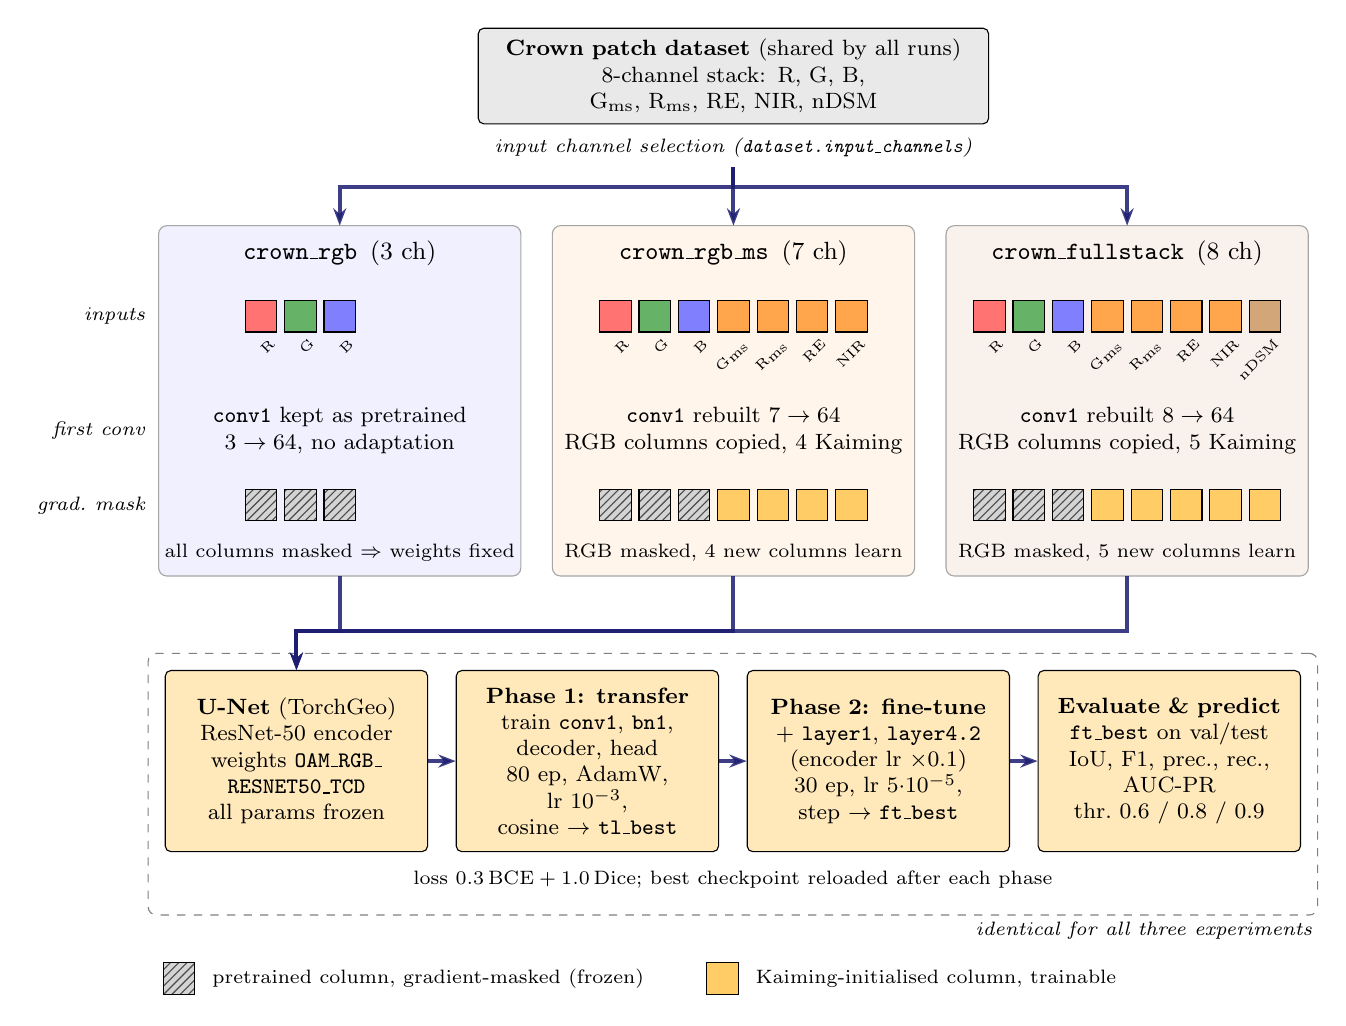
\begin{tikzpicture}[
  font=\footnotesize,
  >={Stealth[length=2.2mm]},
  flow/.style={->, line width=0.5mm, draw=\SkipColor, opacity=0.85},
  box/.style={draw, rounded corners=2pt, align=center, inner sep=4pt},
  stage/.style={box, fill=\ConvColor, fill opacity=0.45, text opacity=1,
               text width=3.05cm, minimum height=2.3cm},
]

% ── data ─────────────────────────────────────────────────────────────────────
\node[box, fill=\InputColor, fill opacity=0.5, text opacity=1, text width=6.2cm]
  (data) at (5,2.3)
  {\textbf{Crown patch dataset} (shared by all runs)\\
   8-channel stack: R, G, B, G$_\mathrm{ms}$, R$_\mathrm{ms}$, RE, NIR, nDSM};
\node[font=\scriptsize\itshape, below=0.05cm of data] (sel)
  {input channel selection (\texttt{dataset.input\_channels})};

% ── three variants ───────────────────────────────────────────────────────────
% lane centres x = 0, 5, 10; rows: title 0, channels -0.9, conv1 -2.0, mask -3.1
\foreach \c/\n/\k in {0/crown\_rgb/3, 5/crown\_rgb\_ms/7, 10/crown\_fullstack/8}{
  \node[font=\small] at (\c,0.05) {\textbf{\texttt{\n}} \,(\k\ ch)};
}

% input channels
\foreach \x/\col/\lab in {-1/chR/R, -0.5/chG/G, 0/chB/B}{ \chip{\x}{-0.75}{\col}{\lab} }
\foreach \x/\col/\lab in {3.5/chR/R, 4/chG/G, 4.5/chB/B,
  5/chMS/G$_\mathrm{ms}$, 5.5/chMS/R$_\mathrm{ms}$, 6/chMS/RE, 6.5/chMS/NIR}{ \chip{\x}{-0.75}{\col}{\lab} }
\foreach \x/\col/\lab in {8.25/chR/R, 8.75/chG/G, 9.25/chB/B,
  9.75/chMS/G$_\mathrm{ms}$, 10.25/chMS/R$_\mathrm{ms}$, 10.75/chMS/RE, 11.25/chMS/NIR,
  11.75/chH/nDSM}{ \chip{\x}{-0.75}{\col}{\lab} }

% first conv
\node[align=center] at (0,-2.2)
  {\texttt{conv1} kept as pretrained\\ $3 \to 64$, no adaptation};
\node[align=center] at (5,-2.2)
  {\texttt{conv1} rebuilt $7 \to 64$\\ RGB columns copied, 4 Kaiming};
\node[align=center] at (10,-2.2)
  {\texttt{conv1} rebuilt $8 \to 64$\\ RGB columns copied, 5 Kaiming};

% gradient mask over conv1.weight input columns
\foreach \x in {-1,-0.5,0}{ \wcol{\x}{-3.15}{1} }
\foreach \x in {3.5,4,4.5}{ \wcol{\x}{-3.15}{1} }
\foreach \x in {5,5.5,6,6.5}{ \wcol{\x}{-3.15}{0} }
\foreach \x in {8.25,8.75,9.25}{ \wcol{\x}{-3.15}{1} }
\foreach \x in {9.75,10.25,10.75,11.25,11.75}{ \wcol{\x}{-3.15}{0} }
\foreach \c/\t in {0/{all columns masked $\Rightarrow$ weights fixed},
                   5/{RGB masked, 4 new columns learn},
                   10/{RGB masked, 5 new columns learn}}{
  \node[font=\scriptsize, align=center] at (\c,-3.75) {\t};
}
\node[font=\scriptsize\itshape, anchor=east] at (-2.35,-3.15) {grad.\ mask};
\node[font=\scriptsize\itshape, anchor=east] at (-2.35,-0.75) {inputs};
\node[font=\scriptsize\itshape, anchor=east] at (-2.35,-2.2) {first conv};

% lane frames
\begin{scope}[on background layer]
  \foreach \c/\f in {0/laneA, 5/laneB, 10/laneC}{
    \draw[rounded corners=3pt, draw=black!35, fill=\f]
      (\c-2.3,0.4) rectangle (\c+2.3,-4.05);
  }
\end{scope}

\draw[flow] (sel.south) -- ++(0,-0.25) -| (0,0.4);
\draw[flow] (sel.south) -- (5,0.4);
\draw[flow] (sel.south) -- ++(0,-0.25) -| (10,0.4);

% ── shared pipeline ──────────────────────────────────────────────────────────
\node[stage] (net) at (-0.55,-6.4)
  {\textbf{U-Net} (TorchGeo)\\ ResNet-50 encoder\\ weights \texttt{OAM\_RGB\_}\\\texttt{RESNET50\_TCD}\\
   all params frozen};
\node[stage, right=0.35cm of net] (tl)
  {\textbf{Phase 1: transfer}\\ train \texttt{conv1}, \texttt{bn1},\\ decoder, head\\
   80 ep, AdamW, lr $10^{-3}$,\\ cosine $\to$ \texttt{tl\_best}};
\node[stage, right=0.35cm of tl] (ft)
  {\textbf{Phase 2: fine-tune}\\ + \texttt{layer1}, \texttt{layer4.2}\\ (encoder lr $\times0.1$)\\
   30 ep, lr $5{\cdot}10^{-5}$,\\ step $\to$ \texttt{ft\_best}};
\node[stage, right=0.35cm of ft] (ev)
  {\textbf{Evaluate \& predict}\\ \texttt{ft\_best} on val/test\\ IoU, F1, prec., rec.,\\ AUC-PR\\
   thr.\ 0.6 / 0.8 / 0.9};
\draw[flow] (net) -- (tl);
\draw[flow] (tl)  -- (ft);
\draw[flow] (ft)  -- (ev);

\node[font=\scriptsize, anchor=north] (loss) at ($(tl.south)!0.5!(ft.south)+(0,-0.12)$)
  {loss $0.3\,\mathrm{BCE} + 1.0\,\mathrm{Dice}$; best checkpoint reloaded after each phase};

\begin{scope}[on background layer]
  \node[draw=black!50, dashed, rounded corners=3pt, inner sep=6pt,
        fit=(net)(tl)(ft)(ev)(loss)] (shared) {};
\end{scope}
\node[font=\scriptsize\itshape, anchor=north east, inner sep=2pt] at (shared.south east)
  {identical for all three experiments};

\foreach \c in {0,5,10}{ \draw[flow] (\c,-4.05) -- (\c,-4.75) -| (net.north); }

% ── legend ───────────────────────────────────────────────────────────────────
\begin{scope}[shift={($(shared.south west)+(0.4,-0.8)$)}]
  \wcol{0}{0}{1}
  \node[font=\scriptsize, anchor=west] at (0.3,0) {pretrained column, gradient-masked (frozen)};
  \wcol{6.9}{0}{0}
  \node[font=\scriptsize, anchor=west] at (7.2,0) {Kaiming-initialised column, trainable};
\end{scope}

\end{tikzpicture}
\end{document}
